\section{Introduction}
\vspace{10pt}

%Cloud vendors offer a lot of different virtual machine instance types. Cloud tenants needs to determine what benefit new virtual machine types will bring to their applications.


Many enterprises are migrating their information technology (IT) needs to public cloud computing platforms, a trend that is projected to continue unabated in the foreseeable future~\cite{forbes}. Among the most important reasons behind these ``tenants'' choosing to procure their IT needs from a public cloud is the promise of lower costs. To effectively realize these cost-related benefits, however, it is crucial that these tenants carry out careful dynamic procurement of IT resources (sometimes labeled ``autoscaling'') to match their evolving needs. Numerous studies show that approaches based on over-provisioning or other ``crude'' estimates of resource needs may negate the cost benefit potential that migrating to a public cloud may offer~\cite{takmig,Li2011,Teregowda10a,Teregowda10b}. Therefore, tenant-side resource procurement has emerged as an area of active research with different aspects of it receiving attention both in  papers~\cite{WuBPKM13,Zafer2012OBS,MenacheSJ14,Zhang15,Farley:2012:MYM:2391229.2391249,DBLP:conf/hotcloud/LeeK11} and industrial products~\cite{cloudphysics,clusterk}. 

Procuring resources cost-effectively from a public cloud %provider 
poses significant technical challenges. One such challenge concerns the problem of determining the set of IT resources (including their capacities) - virtual machines, the virtual network connecting these VMs, storage, etc. - that would be needed to cost-effectively meet the predicted workload of the tenant's software applications while offering satisfactory performance and availability to its users. In order to solve this problem, a tenant must first solve the problem of assessing the performance the users of its application software are likely to experience if the application were assigned a given set of IT resources to meet its predicted workload. Our interest in this paper is in this latter problem, often labeled {\it application performance modeling}~\cite{DBLP:journals/internet/Menasce04,sigmetrics05,Stewart07,SchroederWH06,MiCCS10,ZhangCL14,DBLP:journals/debu/HerodotouB13,DBLP:conf/cmg/MenasceB12}.~\footnote{Of course, application performance modeling has many other uses besides cost optimal resource procurement, e.g., anomaly detection~\cite{Kelly:2005:DPA:1251522.1251530,Cohen:2004:CID:1251254.1251270} and capacity planning~\cite{DBLP:conf/cmg/MenasceN09}.} 

%\noindent{\bf The Problem:} **state the problem.** 

% explain why it is challenging to solve this problem in a public cloud ecosystem
Whereas application performance modeling has been an area of extensive research for many decades across many communities, solving it for the public cloud ecosystem presents a tenant with non-trivial novel sources of complexity. In particular, most modeling solutions have traditionally been developed for settings involving privately owned and operated data centers or clusters. These solutions may not be readily adapted to a public cloud. %A typical example of such a private setting is a data center or a cluster privately owned and operated by an enterprise that is considering replacing it in favor of a move of its IT needs to a public cloud. 

\begin{figure}[htbp]
\centering
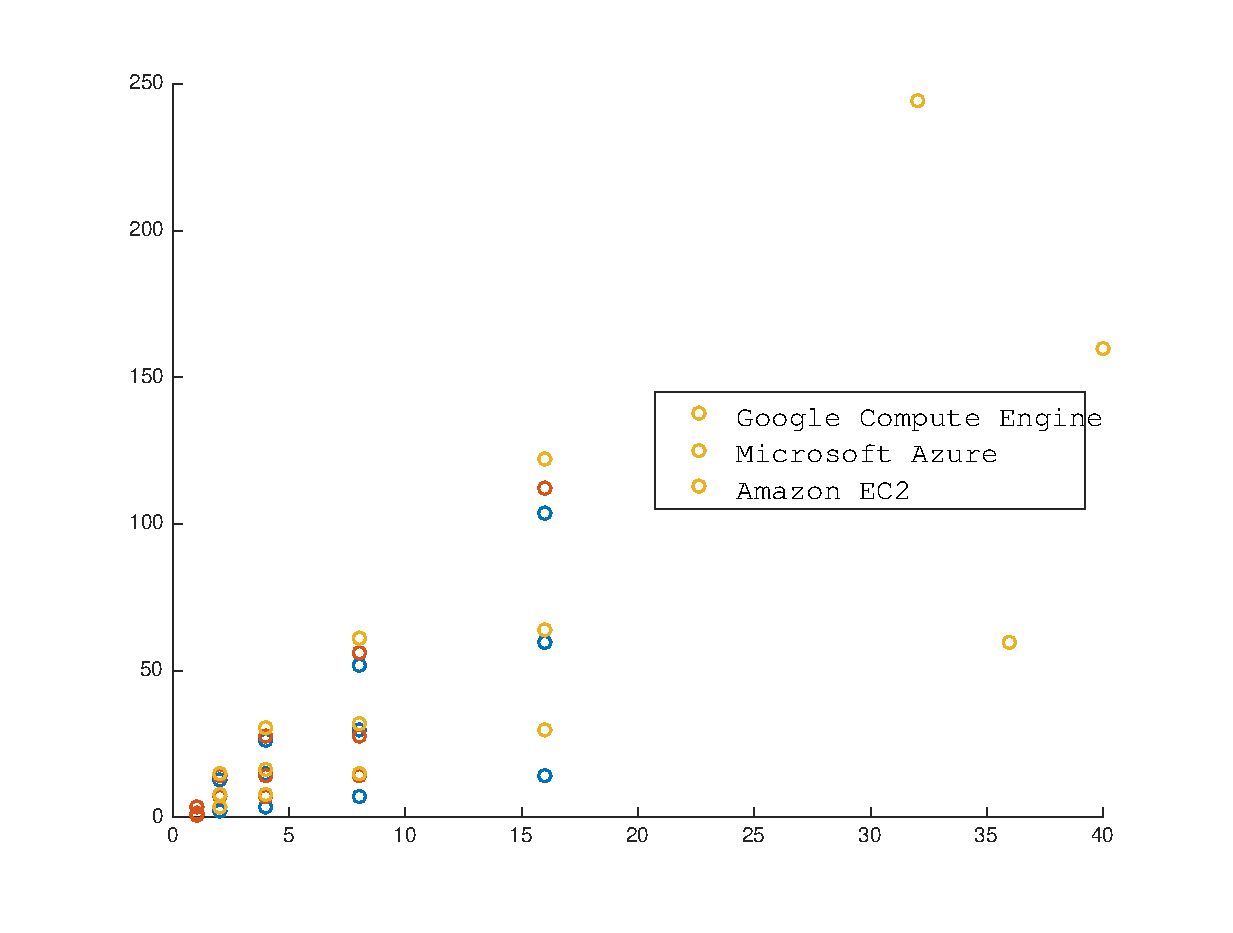
\includegraphics[width=0.45\textwidth]{cloud_vm_types.eps}
\caption{An illustration of the diversity in VM capacities offered by popular public cloud providers. We show VMs with a wide range of CPU and memory capacities offered by Amazon EC2~\cite{amazon-ec2}, Google Compute Engine~\cite{google-computeengine}, and Microsoft Azure~\cite{windows-azure}. The number of cores on these VMs ranges from 1 to 32 whereas their memory capacity ranges from 0.75GB to 256GB.} \label{fig:diversity}
%\vspace{-10pt}
\end{figure}


%Arguably, the most important 
One of the most important differences between  these two settings (from the point of view of application performance modeling) is the immense {\it diversity of resources} that a typical public cloud offers.~\footnote{There are other important differences complementary to our focus in this paper and part of our future work. E.g., in a private setting, the user of a machine (tenant application) coincides with its owner while in a public setting the two are separated via virtualization techniques with implications for how much information about physical resource usage is available to the tenant's models. } We focus on virtual machines (VMs) %as the resource type of interest 
in this work although our arguments likely apply to other resource types as well. To appreciate this diversity, let us consider some examples from the most prominent public cloud providers that offer many VM types since they need to cater to many different types of customers. Here VM instance types are organized into groups based on use case.  Instances within a group generally have the same CPU generation and clock speed, and vary by the number of CPUs and memory.  Amazon EC2 offers over 40 VM types organized into eight different groups, varying in CPU, memory, network bandwidth, storage speed, and pricing~\cite{amazon-ec2}. Google Compute Engine offers 15 instance types organized into four groups: Standard, High CPU, High Memory, and Shared Core (for lightweight applications)~\cite{google-computeengine}. Finally, Microsoft Azure offers 30 instance types organized into 4 groups~\cite{windows-azure}. Figure~\ref{fig:diversity} shows 44 VM instance types from these three providers capturing the large spectrum of CPU cores and memory that their VMs pack. %organized into four groups: Basic, Standard, Optimized, and Optimized (version 2).

A typical privately owned data center, on the other hand, is likely to possess a much smaller number of machine types. Keeping machines (and their software configurations) relatively homogeneous brings about significant benefits related to ease of system administration and cost savings (e.g., due to bulk purchase offers from IT vendors). Although factors such as incremental procurement over time, meeting specialized needs (e.g., machines with GPUs), etc.,  do result in some differences among machine types even in a private data center, the overall degree of heterogeneity is significantly smaller than that seen in a  public cloud.

This high diversity of resource types in a public cloud introduces an additional source of complexity into a tenant's %decision-making related to 
VM autoscaling decision-making. Since the number of machine types in traditional IT environments is small and relatively fixed, performance models have conventionally been developed and calibrated using performance measurements (``profiling'') on the same/similar type of machines on which the application would eventually execute. On the other hand, a tenant of a public cloud would be interested in being able to predict the performance that its workload might experience on a wide variety of VM types that the provider offers. This is because which VM types are the most cost-effective for a tenant's workload might change over time due to: (i) changes in the tenant's own workload (e.g., many applications show periodic time-of-day or seasonal variations in their workload intensities) and (ii) dynamism and variety in the cloud provider's pricing schemes (e.g., Amazon EC2 offers spot pricing for most of its instance types and such spot instances are usually much cheaper than their on-demand counterparts). Additionally, existing work also shows that even during a period of stationary workload, procuring heterogeneous VMs (e.g., a combination of ``small'' and ''large'') can often offer a better cost vs. performance trade-off than procuring the same types of VMs (e.g., a larger number of only ``small'' or a smaller number of only ''large'')~\cite{Zhang15}
Clearly, approaches based on calibrating a tenant's performance models separately on the dozens of resource types that public clouds offer are likely to not scale well. Furthermore, such approaches may prove to be expensive, defeating the original intent of cost-efficacy!

% introduce the idea of exploiting diversity instead of letting it be a hindrance. 
We wish to explore if a tenant might actually be able to benefit from this diversity by deliberately and carefully exploiting it to ease the creation and calibration of its application performance models. The intuition underlying our premise is that choosing a small subset of the offered VMs may suffice for calibrating a tenant's performance models well if this subset were chosen carefully. In particular, this subset should capture well the overall diversity across the VMs offered by the provider. 

%*** explain why we expect this to be the case. *** This leads us to explore the following hypothesis: {\it diversity of VMs in a public cloud can aid in making the calibration of tenant application performance models on unseen VMs more scalable and affordable.} 

%An important aspect of our hypothesis worth highlighting is that it is not tied to a specific performance modeling approach. ** expand this **

\begin{figure*}[htbp]
\centering
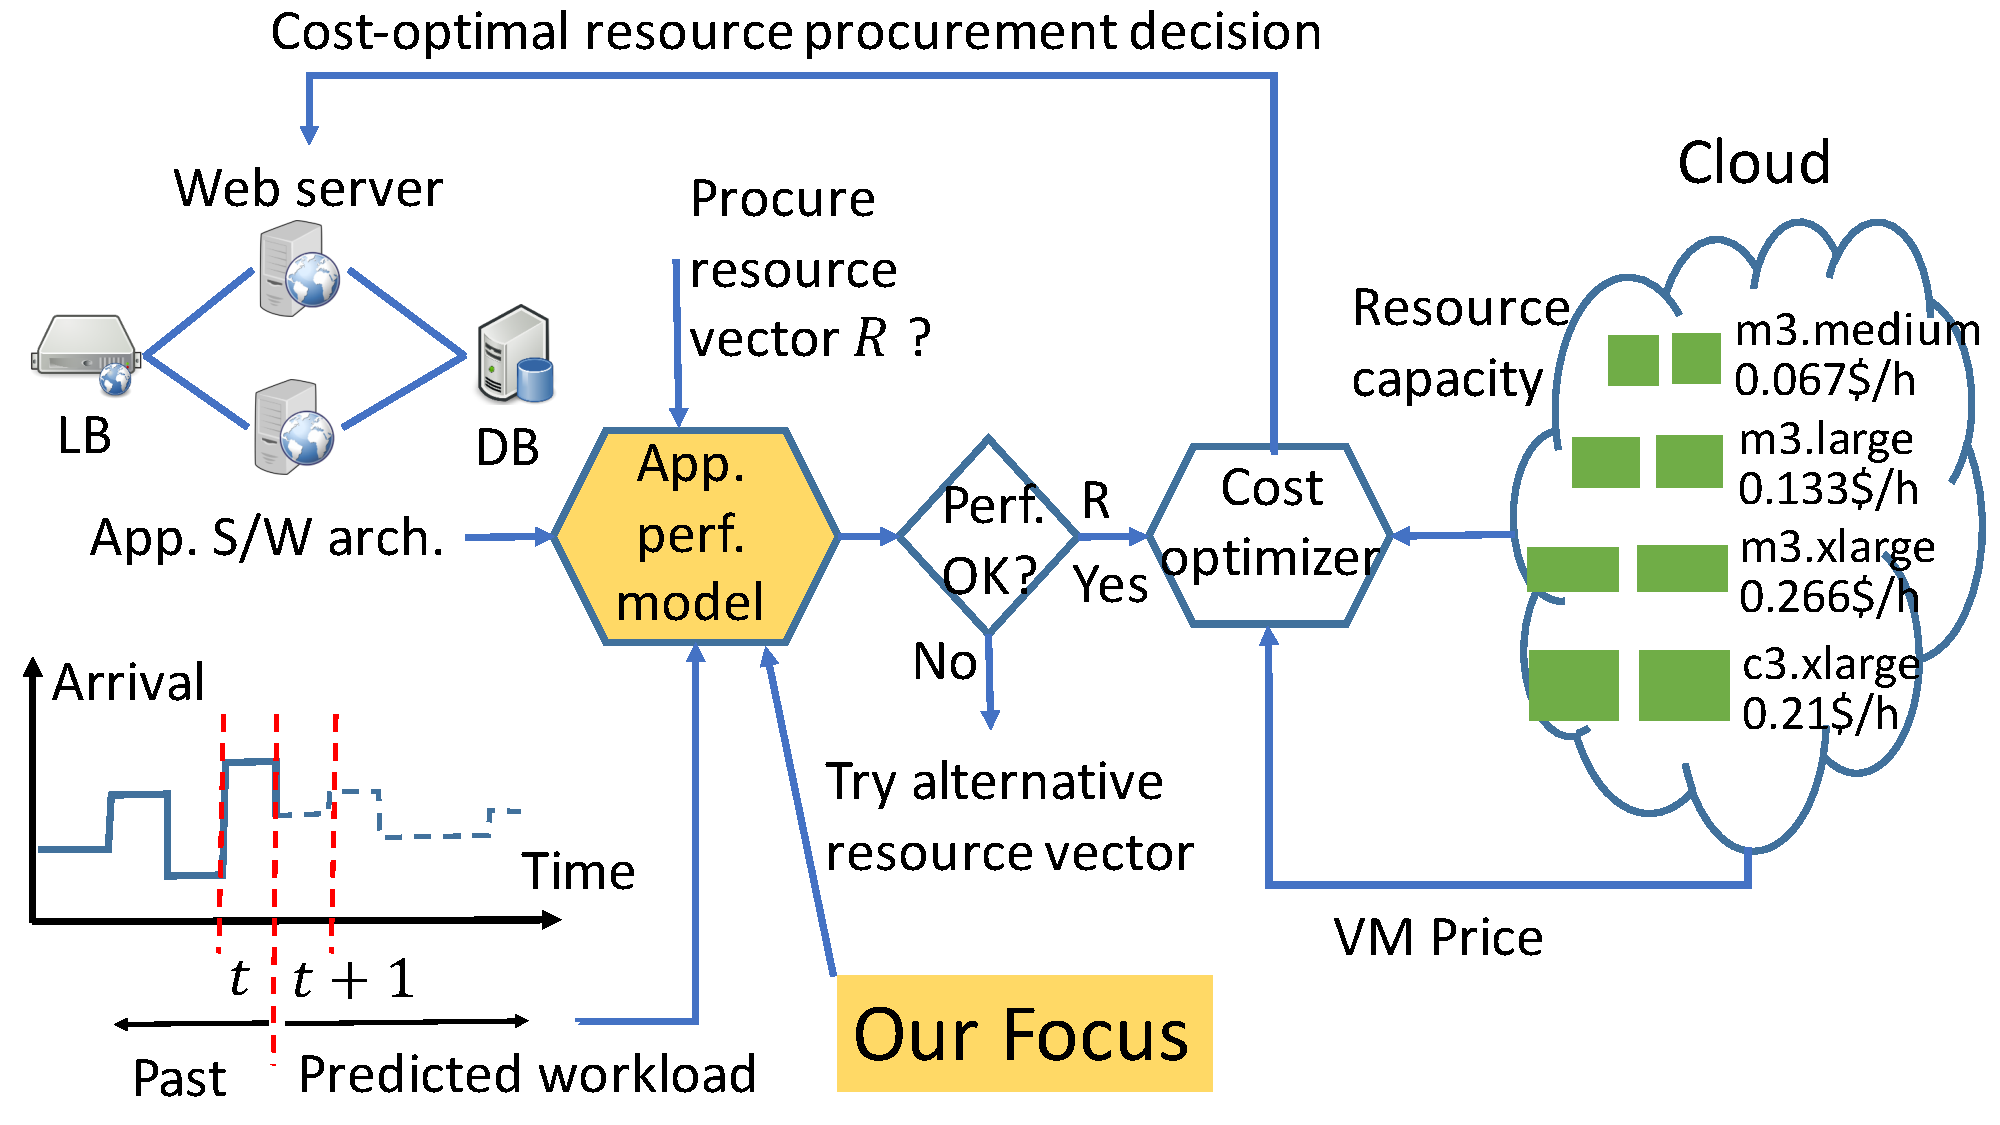
\includegraphics[width=0.8\textwidth]{system}
\caption{An overview of interactions between the performance modeling problem we study and other aspects of the overall decision-making for a cost-conscious tenant procuring resources from a public cloud. The example VM types and their prices shown are chosen from Amazon EC2. }
\label{fig:diagram}
%\vspace{-10pt}
\end{figure*}


\noindent {\bf Our Approach and Contributions:} In this paper, we take a small first step towards exploring the above idea by evaluating the following hypothesis: {\em using a more diverse set of VMs for calibrating/training a performance model helps improve its accuracy}. Specifically, we devise a multiple linear regression modeling framework for predicting the performance of interactive data  serveing applications. We calibrate this model for three different types of real-world applications: (i) Redis~\cite{redis}, an open-source in-memory NoSQL key-value store, (ii) Apache Cassandra~\cite{cassandra}, a Table/key-value hybrid NoSQL database, and (iii) MySQL, a popular open-source ACID database~\cite{mysql}. We use ``training sets'' of varying sizes (i.e., numbers of VM types) for our calibration and investigate the impact of the training set size on model efficacy. Our results are promising. E.g., for Redis, we find that the $R^2_{predicted}$ measure of model efficacy improves from 0.4-0.5 with 2 VM types for training and 0.7 with 3 VM types to 0.8 for 4 VM types. 
%\begin{itemize}
%\item ...
%\item ...
%\item ...
%\end{itemize}

Whereas the benefits of exploiting heterogeneity have been explored in other contexts (most notably for cost/performance optimization in cloud settings~\cite{DBLP:conf/cloud/ReissTGKK12,Zhang15,Farley:2012:MYM:2391229.2391249,DBLP:conf/hotcloud/LeeK11}), to the best of our knowledge, our paper is the first to systematically explore its role in aiding performance model calibration. %On the one hand, o
Our work is highly complementary to traditional performance modeling research. At the same time, it opens up a promising new area for further exploration. As part of our own future work, we plan to investigate if/how public cloud providers could offer ``performance modeling as a service,'' whereby all/many aspects of the model calibration by exploiting diversity would be offered as an automated facility to their tenants. 
%... ** discuss the possibility of offering PMaaS as a key implication of our work as well as being an interesting direction for future research. **



The rest of this paper is organized as follows. In Section~\ref{sec:back}, we provide an overview of a generic cost-conscious tenant's decision-making and where application performance modeling fits within it.  In Section~\ref{sec:model}, we describe the performance modeling techniques that we employ.  In Section~\ref{sec:eval}, we present our empirical evaluation of our hypothesis using three real-world applications as our case studies. We discuss related work in Section~\ref{sec:related}.  Finally, %we discuss unresolved challenges and future directions in Section~\ref{sec:future} and conclude 
present concluding remarks in Section~\ref{sec:conclus}. 
 

%Solution: test your application on different VM types and find out?

%present the problem, its significance, and key challenges
 
%explain why the state-of-the-art may not be adequate, particularly as clouds move towards higher levels of utilization and dynamism

%explain our key ideas and contributions
